\documentclass{article}
\usepackage[margin=2.5cm, top=4cm, headheight=25pt]{geometry}
\usepackage{amsmath, amssymb, enumitem, fancyhdr, graphicx}
\usepackage[indent=20pt]{parskip}
\usepackage[hidelinks]{hyperref}
\usepackage{xcolor}
\usepackage{listings}
\usepackage{subcaption}
\usepackage{url}
\usepackage[most]{tcolorbox}
\usepackage{lastpage}

\tcbuselibrary{listingsutf8} % Support for lstlistings within tcolorbox

\newtcolorbox[auto counter, number within=section]{question}[1][]{%
    colframe=gray!80,                      % Dark gray frame
    colback=gray!5,                       % Light gray background
    coltitle=black,                        % Black title
    title=\textbf{Question~\thetcbcounter}, % Bold title
    fonttitle=\bfseries\large,             % Subtle title font size
    rounded corners,                   % Slightly more rounded corners
    boxrule=0.25mm,                         % Thinner border for a sleek look
    enhanced,                              % Enhanced box features
    attach boxed title to top left={xshift=2mm, yshift=-2mm},
    boxed title style={colframe=gray!80, colback=gray!5, boxrule=0.25mm},
    % Title styling
    #1
}

\bibliographystyle{IEEEtran}
\graphicspath{{./images/}}

% -- Custom Variables --
\def\me{Rajdeep Gill (7934493)}
\def\partner{Daniyal Hasnain (7942244)}
\def\course{ECE 4830}
\def\labsection{B03}
\def\labno{4}
\def\title{Lab 4}

% -- Styling for code snippets --
\lstset{
    basicstyle=\ttfamily\small,           % Basic font style
    keywordstyle=\color{blue},            % Keywords color
    commentstyle=\color{gray},            % Comments color
    stringstyle=\color{teal},             % Strings color
    numbers=left,                         % Line numbers on the left
    numberstyle=\tiny\color{gray},        % Line number style
    stepnumber=1,                         % Line number step
    numbersep=10pt,                       % Space between line numbers and code
    backgroundcolor=\color{lightgray!10}, % Background color
    frame=single,                         % Adds a frame around the code
    breaklines=true,                      % Line breaking for long lines
    captionpos=b,                         % Caption position
    showspaces=false,                     % Don't show spaces
    showstringspaces=false                % Don't show spaces in strings
}
\renewcommand{\lstlistingname}{Code Snippet}

\renewcommand{\arraystretch}{1.2} % For less-ugly tables
\setlength\parindent{0pt}

%----- Samples 
% Questions:
%   \begin{question}[title=Custom Question Title]
%       Question details
%   \end{question}

% Tables:
%   \begin{table}[htbp]
%       \centering
%       \caption{Table Caption}
%       \begin{tabular}{ll}
%           \toprule
%           \textbf{Column 1} & \textbf{Column 2} \\
%           \midrule
%           Row 1 & Row 2 \\
%           Row 3 & Row 4 \\
%           \bottomrule
%       \end{tabular}
%   \end{table} 

% Figures:
%   Single figure:
%       \begin{figure}[htbp]
%           \centering
%           \includegraphics[width=0.5\textwidth]{example-image}
%           \caption{Figure Caption}
%       \end{figure}
%   Multiple figures:
%       \begin{figure}[htbp]
%           \centering
%           \begin{subfigure}[b]{0.5\textwidth}
%               \includegraphics[width=\textwidth]{example-image-a}
%               \caption{First subfigure}
%           \end{subfigure}
%           \begin{subfigure}[b]{0.5\textwidth}
%               \includegraphics[width=\textwidth]{example-image-b}
%               \caption{Second subfigure}
%           \end{subfigure}
%           \caption{Main figure}
%       \end{figure}

\begin{document}

% --------------------------------------------------------------------------------
% TITLE
% --------------------------------------------------------------------------------

\begin{center}
    \huge \title

    \vspace{2mm}
    \hrule

    \vspace{4mm}
    \large \me ~\&~\partner

    \vspace{2mm}
    \large \course~\labsection

    \vspace{2mm}
    \today
\end{center}

\vspace{4mm}

% --------------------------------------------------------------------------------
% END TITLE
% --------------------------------------------------------------------------------

\newpage

\tableofcontents

\vspace{1cm}
\newpage

\pagestyle{fancy}
\fancyhead[L]{\large Lab \labno}
\fancyhead[R]{\large \me, \partner}

\fancyfoot[C]{Page \thepage~of~\pageref{LastPage}}

% --------------------------------------------------------------------------------
% BODY
% --------------------------------------------------------------------------------

\section{Problem 1}

There is a distinct noise when playing the audio overlapping the tune. We can use a simple mask to eliminate this single sinusoidal tone. First, we plot the FFT before any filtering to detect the noise frequency. Since the audio is stereo, we can work with just the left side (as they are near-identical). The plot below shows the magnitude spectrum before filtering:

\begin{figure}[h]
    \centering
    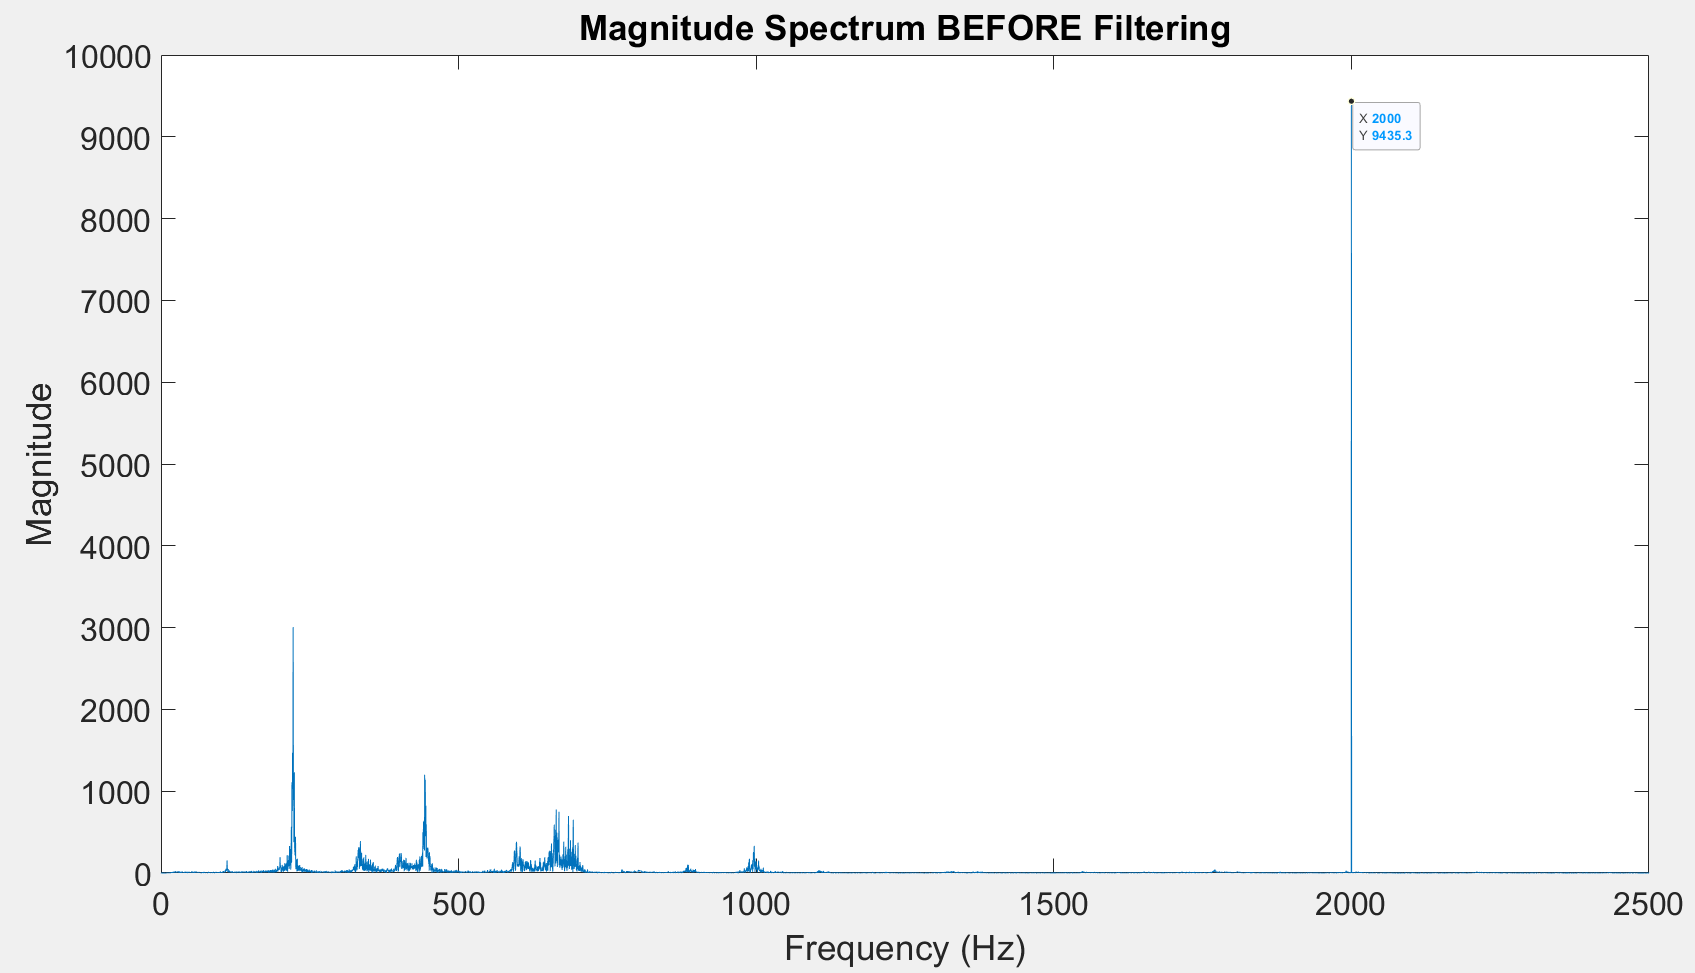
\includegraphics[width=0.5\textwidth]{P1_before_filtering.png}
    \caption{Magnitude spectrum of the given audio's left side before filtering.}
    \label{fig:p1_before_filtering}
\end{figure}

A quick scan shows a distinct peak at 2000 Hz\textemdash the noise we seek to remove. A straightforward notch filter implemented as a binary mask will do the trick; we set the mask to an array of ones except at the index that corresponds to 2000 Hz, where we set zeroes. Multiplying the data vector with this mask will effectively remove the noise. To get the bin index for the observed noise, we use:
\[
\text{Index} = \frac{\text{Noise Frequency} \times N}{F_s} = \frac{2000 \times 132300}{44100} = \textbf{6000}
\]
To account for small numerical errors in rounding and/or leakage, we can set a small margin of error around this index to set to zero (5995-6005 is sufficient). The snippet below shows the filter used in Matlab code:

\begin{lstlisting}[language={MATLAB}, label={code:p1}, caption={Notch Filter}]
% notch filter
mask = ones(N, 1);
notch_range = 5;  % small margin for errors
% Remove the detected frequency with its margin
mask(index-notch_range:index+notch_range) = 0; % set 5995-6005 to zero
mask(N-(index+notch_range):N-(index-notch_range)) = 0; % symmetric pair
\end{lstlisting}

Multiplying the left and right sides by the mask, taking the inverse FFT (ifft), and plotting the combined waveform gave the following wave seen in \autoref{fig:p1_after_filtering}. As we can see, the noise-peak at 2000 Hz is now gone, leaving us with the filtered audio. Listening to the output confirms the result. At this point, we used only the FFT and designed a simple notch filter (binary mask) to eliminate the single sinusoidal tone successfully.


\begin{figure}[ht!]
    \centering
    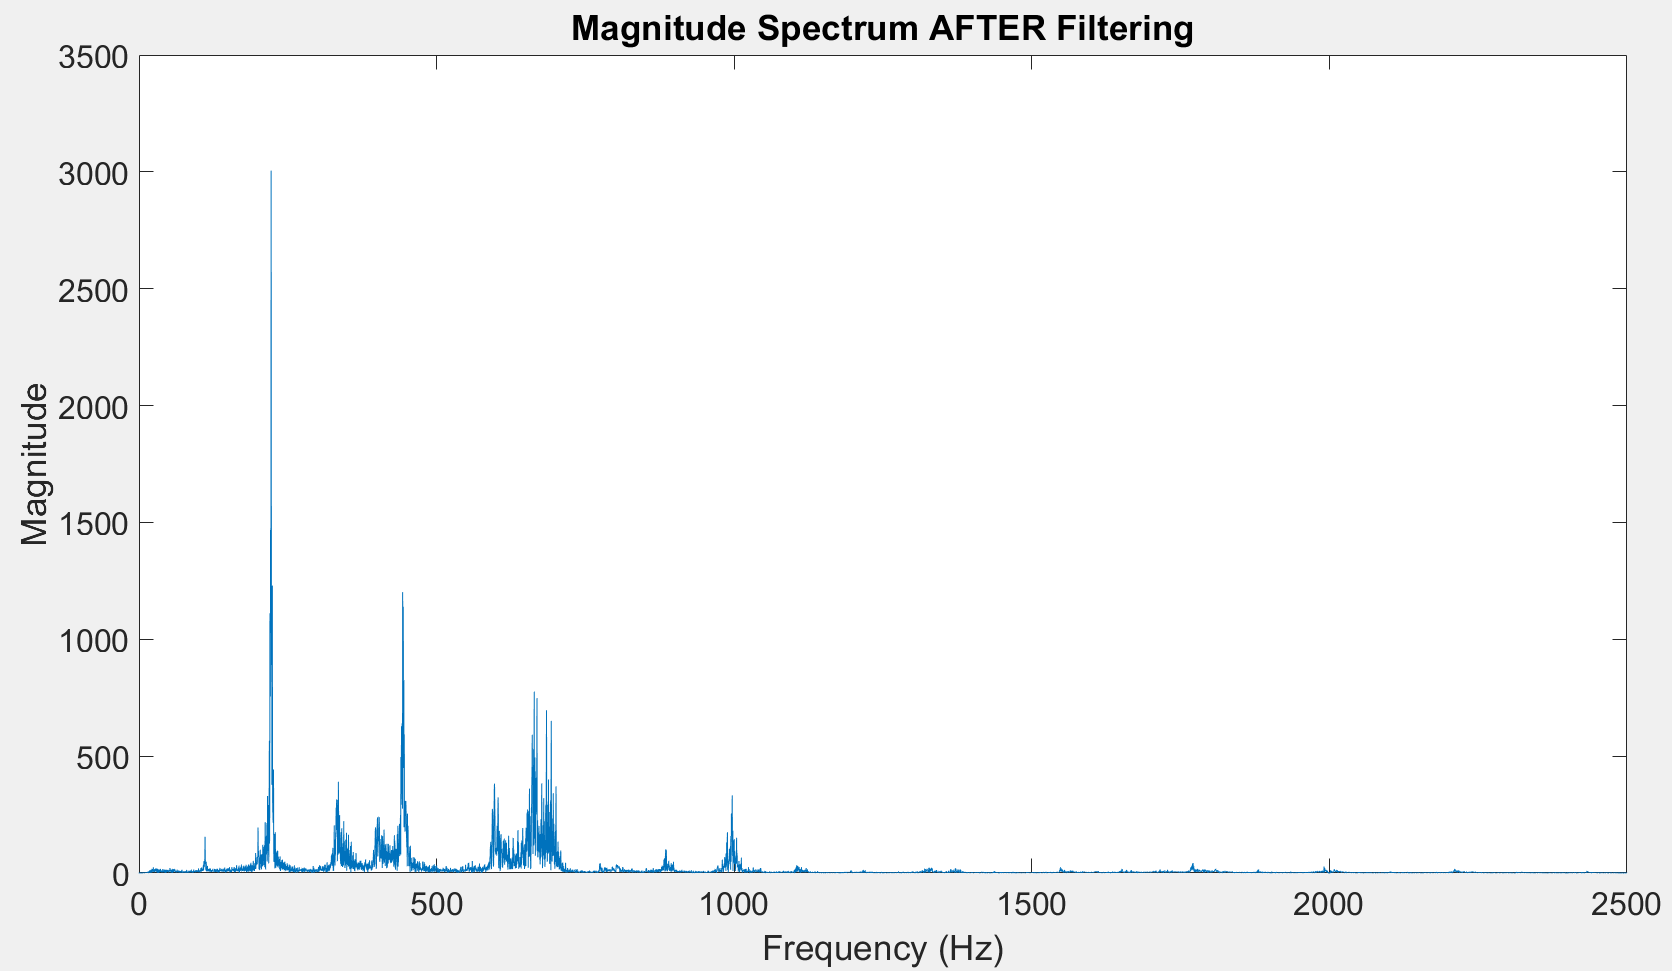
\includegraphics[width=0.5\textwidth]{P1_after_filtering.png}
    \caption{Magnitude spectrum of the given audio's left side after filtering.}
    \label{fig:p1_after_filtering}
\end{figure}


\newpage
\section{Problem 2}

To remove the water interaction with the hydrophone, we first find the STFT (Short-Time Fourier Transform) of the audio. We can then try to filter out all the noise by using an threshold filter. The STFT plotted in the decibel scale is shown in \autoref{fig:p2}.
\begin{figure}[ht!]
    \centering
    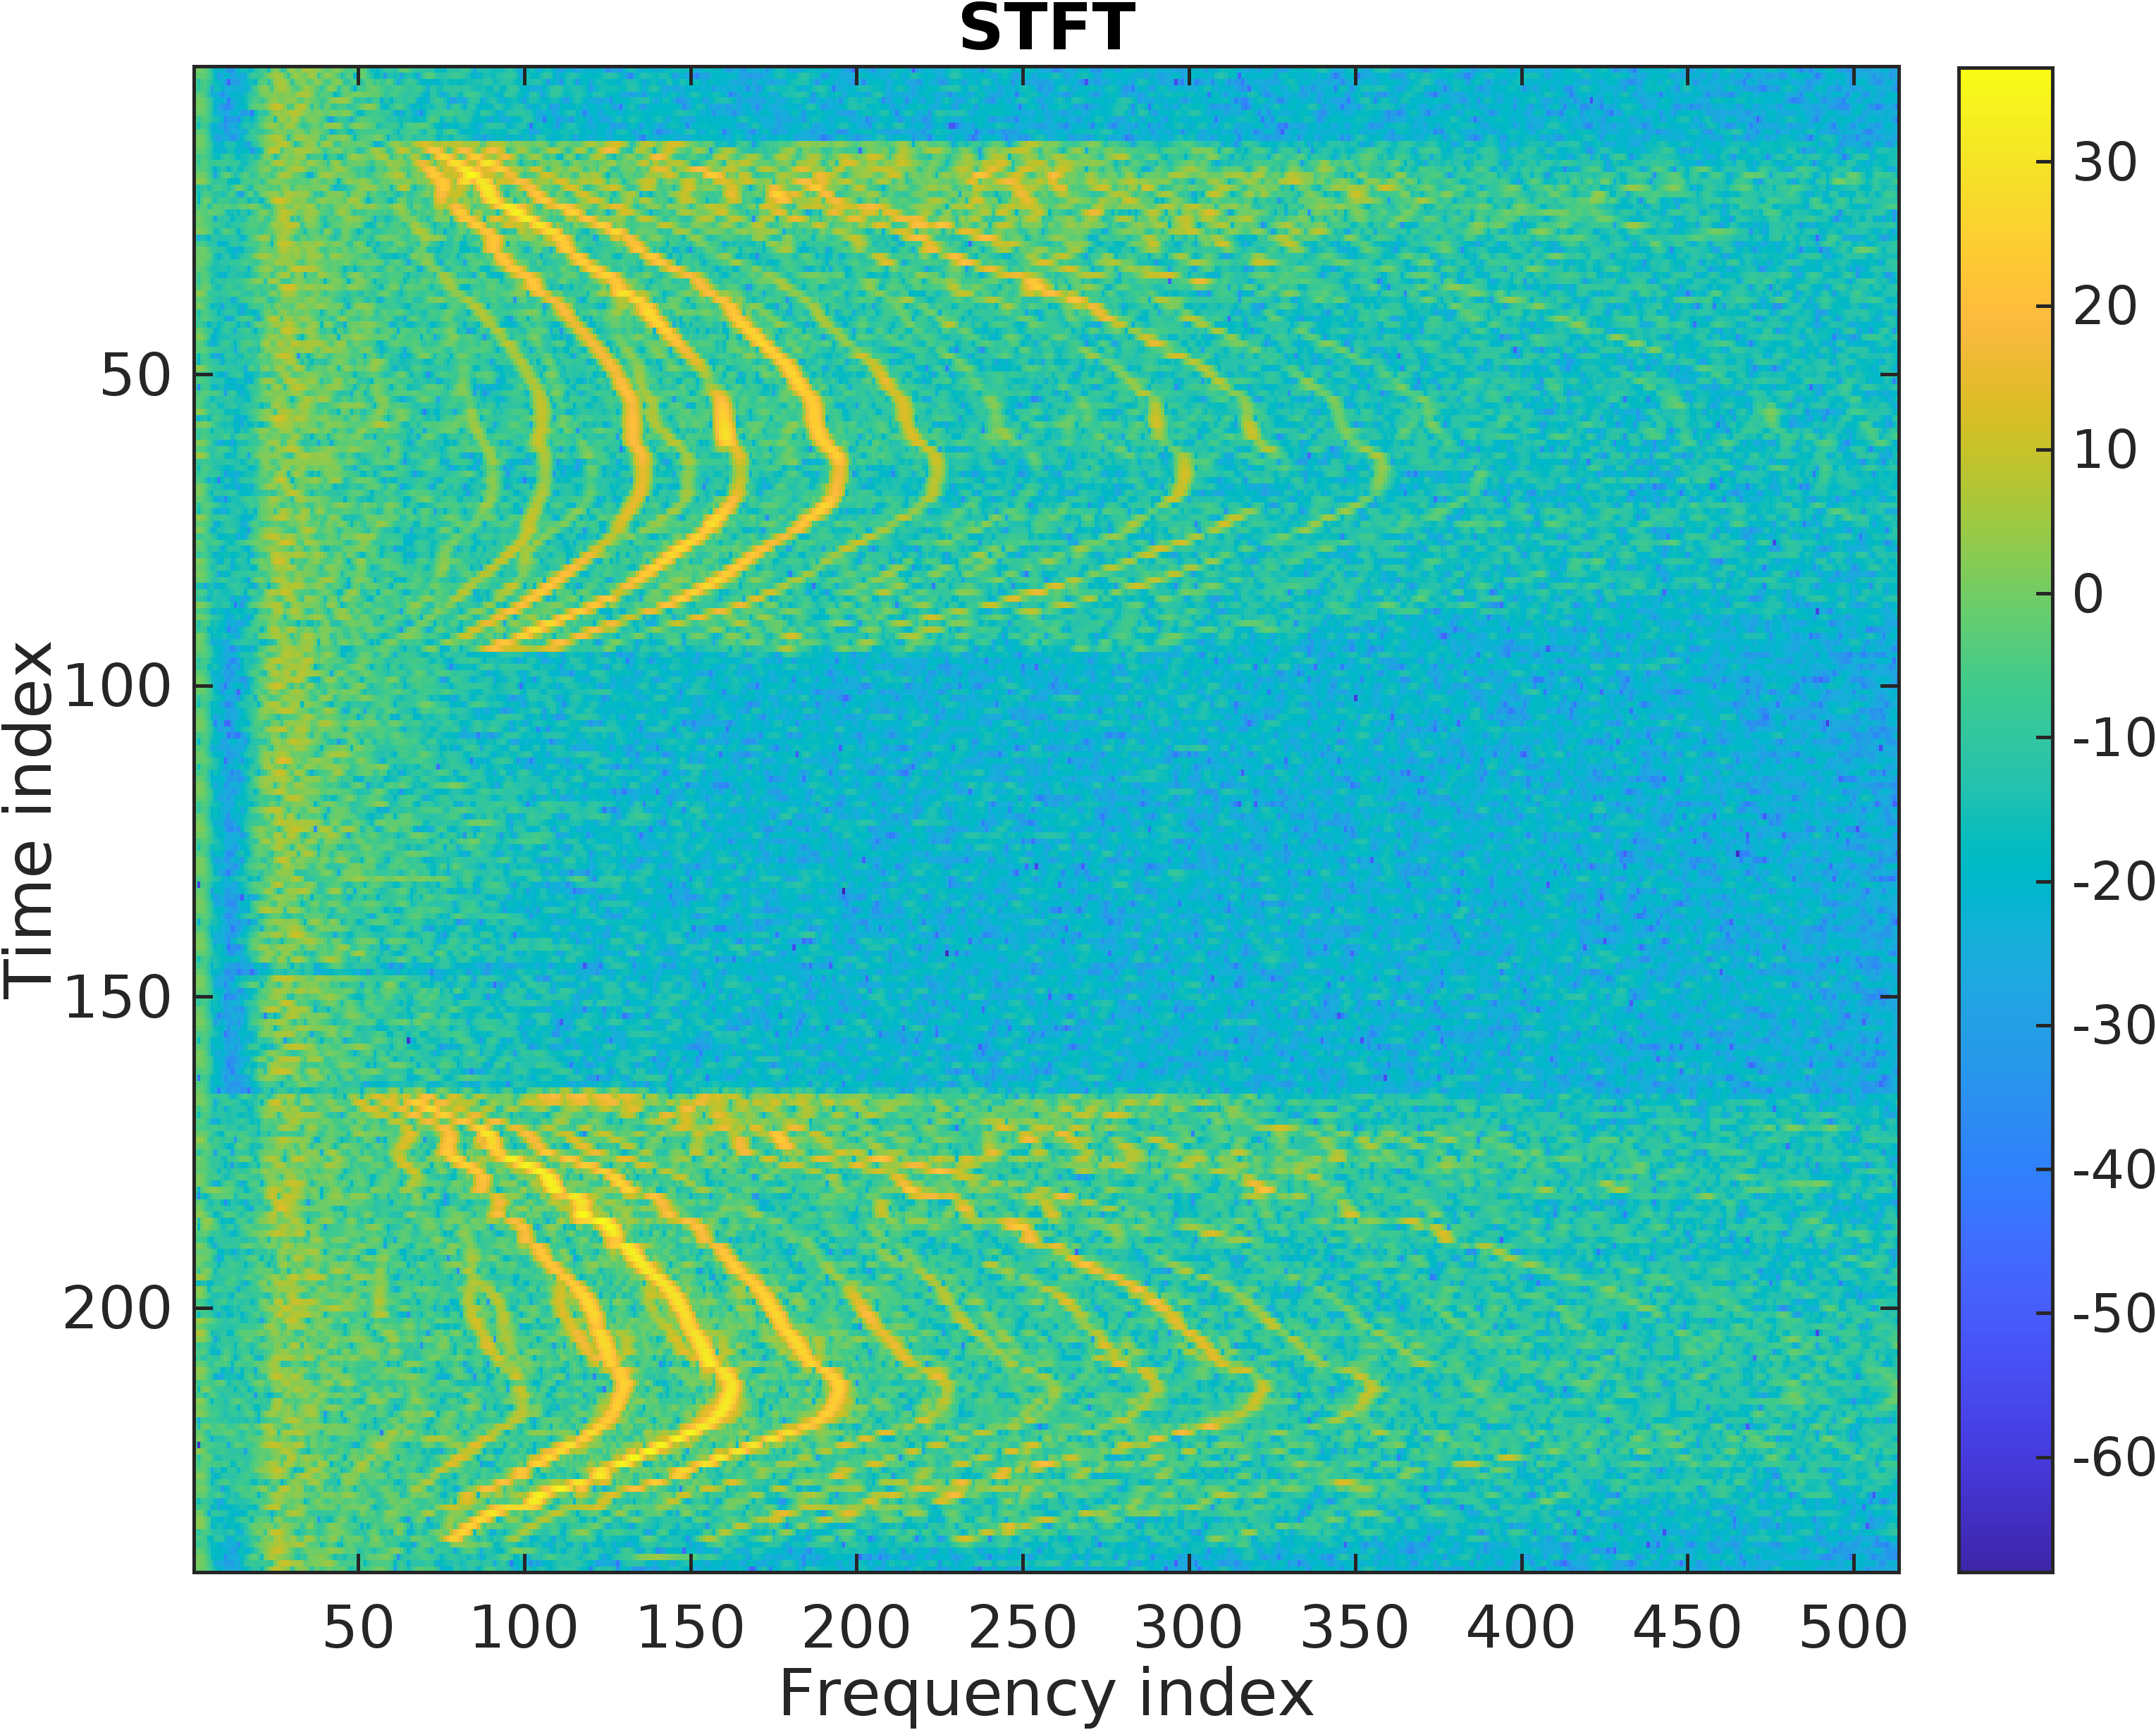
\includegraphics[width=0.5\textwidth]{p2.png}
    \caption{STFT of the given audio before filtering.}
    \label{fig:p2}
\end{figure}

We notice that the values below 6 are mostly noise and the most prominent waveforms have a much higher ampltitude. We can use this information to filter out the noise. The code snippet below shows the filtering process:
\begin{lstlisting}[language={MATLAB}, label={code:p2}, caption={Threshold Filter}]
    [audio, fs] = audioread("Globicefalo_clip.wav");
    fft_length = 1024;       % FFT length
    win_length = 512;        % Window length
    time_res = 512;          % Time resolution (hop size)
    X = STFT(audio, fft_length, win_length, time_res);
    thresh = 6;
    X_mag = abs(X);
    X_filtered = X;
    X_filtered(X_mag < thresh) = 0;
\end{lstlisting}
This is a simple binary threshold filter that sets all values below 6 to zero, the plot of the filter is shown in \autoref{fig:p2_threshold}.
\begin{figure}[ht!]
    \centering
    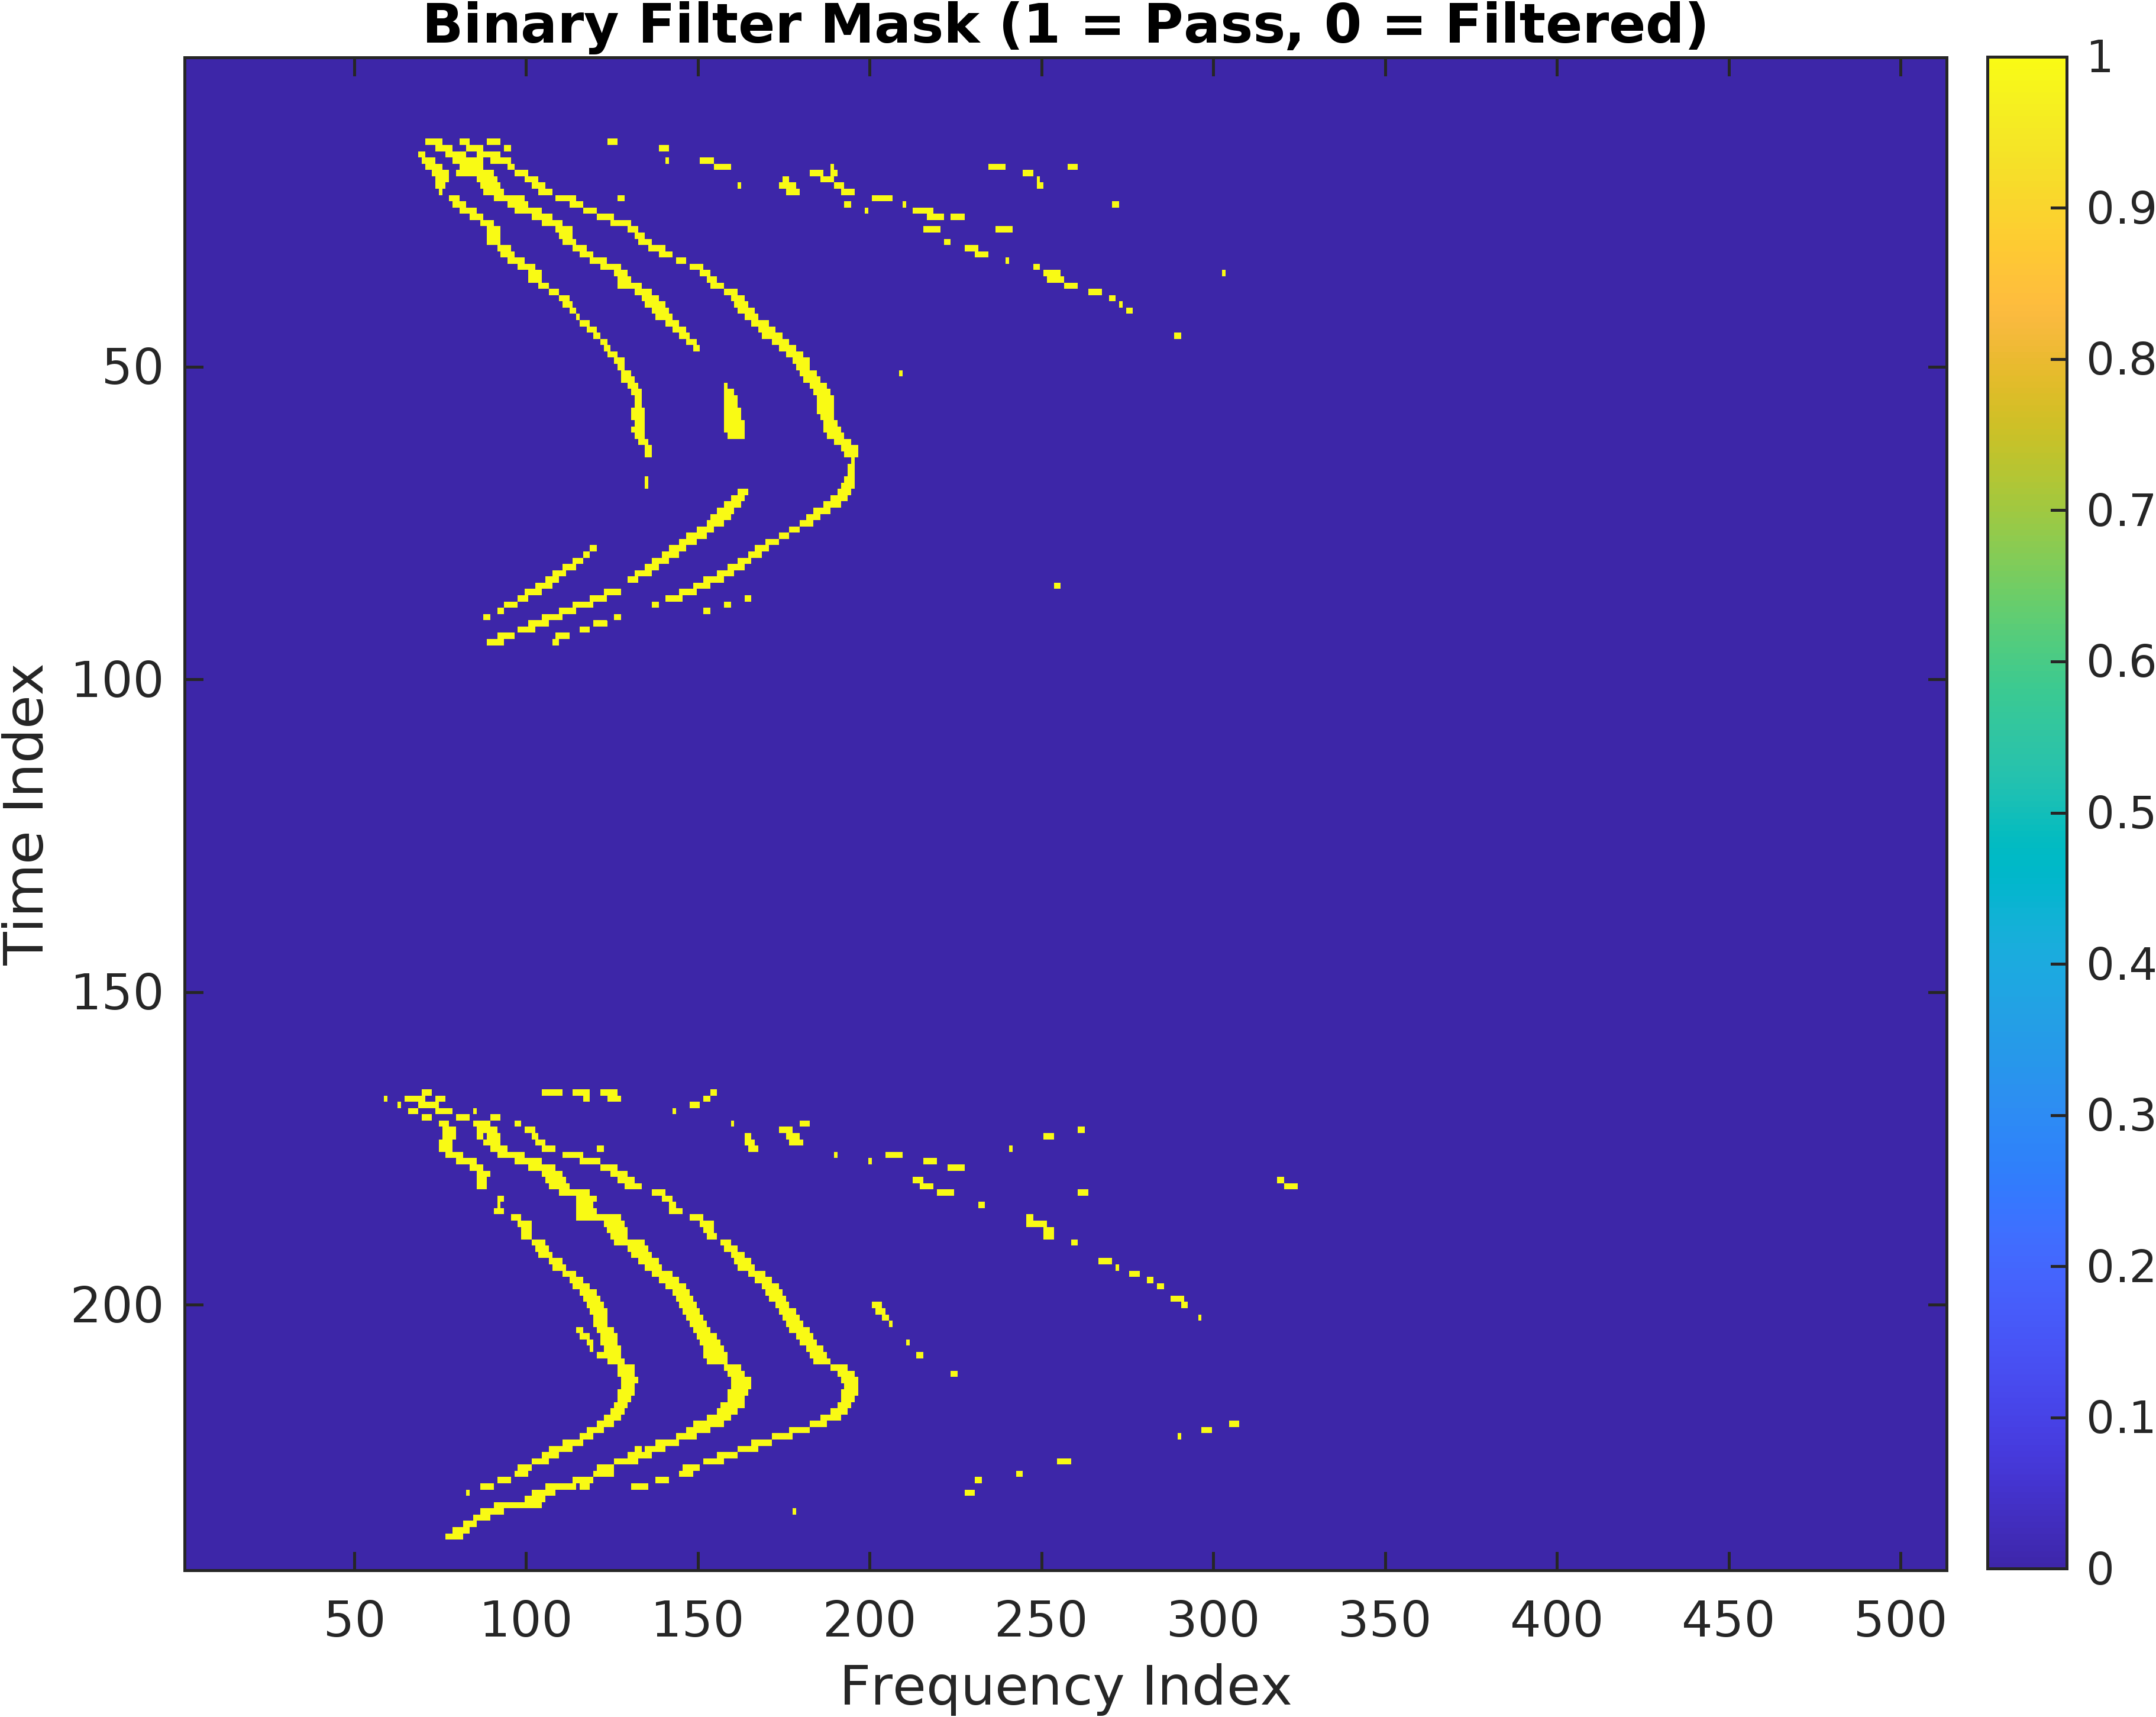
\includegraphics[width=0.5\textwidth]{filter.png}
    \caption{Threshold filter used to filter out the noise.}
    \label{fig:p2_threshold}
\end{figure}

The STFT of the audio after filtering is shown in \autoref{fig:p2_filtered}.
\begin{figure}[ht!]
    \centering
    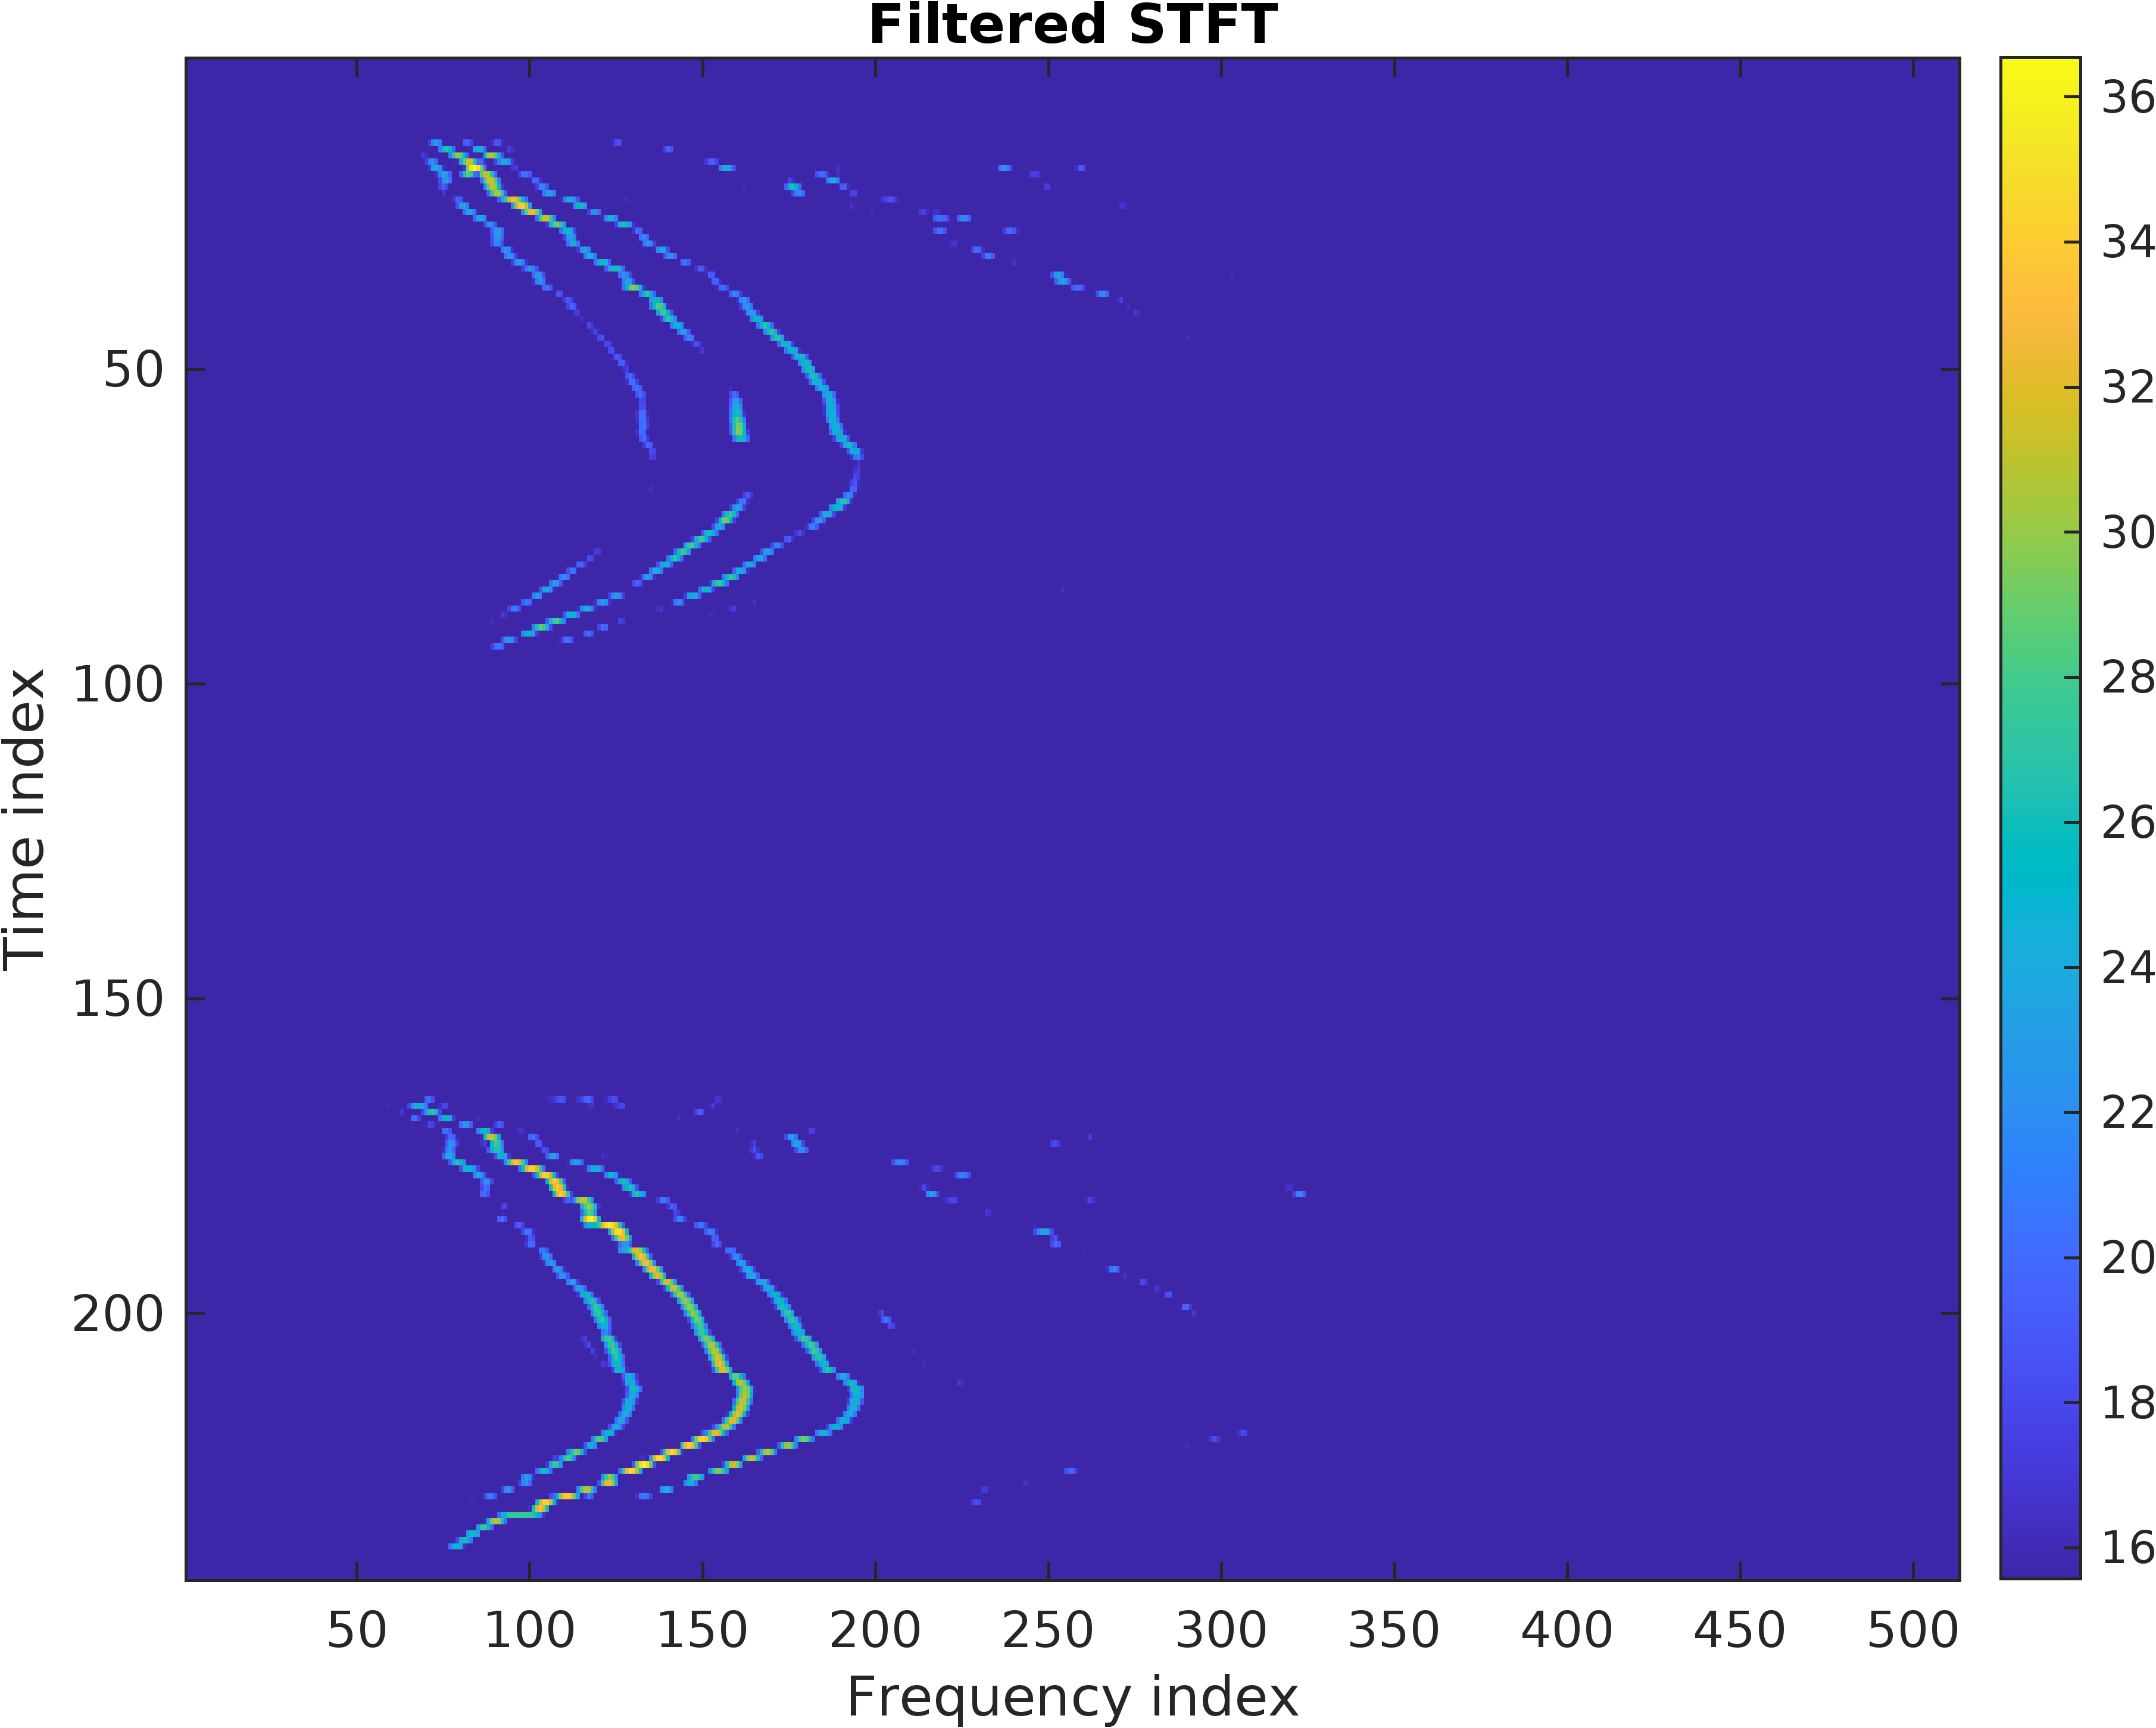
\includegraphics[width=0.5\textwidth]{filtered_signal.png}
    \caption{STFT of the given audio after filtering.}
    \label{fig:p2_filtered}
\end{figure}

Listening to both audios, we see that the filtered audio has no water-interaction noise and only contains the sound of the sea-creature.

% --------------------------------------------------------------------------------
% END BODY
% --------------------------------------------------------------------------------

\end{document}
